\documentclass{article}

\usepackage{titlesec}
\usepackage{titling}
\usepackage{graphicx}
\graphicspath{ {writeupimages/} }
\usepackage{float}

\titleformat{\section}
{\Large\bfseries}
{}
{0em}
{}[\titlerule]

\titleformat{\subsection}
{\large\bfseries}
{}
{0em}
{}

\titleformat{\subsubsection}
{\bfseries}
{}
{0em}
{}


\begin{document}

\title{Project: Perception Pick \& Place}
\author{Brett Gleason}

\maketitle

The rubric for this project can be found at the following URL: \\
https://review.udacity.com/\#!/rubrics/1067/view \\
I will consider the rubric points individually and describe how I addressed each point in my implementation.

\subsubsection{Required Steps for a Passing Submission:}

\begin{enumerate}
    \item 1. Extract features and train an SVM model on new objects (see `pick\_list\_*.yaml` in `/pr2\_robot/config/` for the list of models you'll be trying to identify). 
    \item 2. Write a ROS node and subscribe to `/pr2/world/points` topic. This topic contains noisy point cloud data that you must work with.
    \item 3. Use filtering and RANSAC plane fitting to isolate the objects of interest from the rest of the scene.
    \item 4. Apply Euclidean clustering to create separate clusters for individual items.
    \item 5. Perform object recognition on these objects and assign them labels (markers in RViz).
    \item 6. Calculate the centroid (average in x, y and z) of the set of points belonging to that each object.
    \item 7. Create ROS messages containing the details of each object (name, pick\_pose, etc.) and write these messages out to `.yaml` files, one for each of the 3 scenarios (`test1-3.world` in `/pr2\_robot/worlds/`).  See the example `output.yaml` for details on what the output should look like.  
    \item 8. Submit a link to your GitHub repo for the project or the Python code for your perception pipeline and your output `.yaml` files (3 `.yaml` files, one for each test world).  You must have correctly identified 100\% of objects from `pick\_list\_1.yaml` for `test1.world`, 80\% of items from `pick\_list\_2.yaml` for `test2.world` and 75\% of items from `pick\_list\_3.yaml` in `test3.world`.
    \item 9. Congratulations!  You're done!
\end{enumerate}



% # Extra Challenges: Complete the Pick & Place

% 7. To create a collision map, publish a point cloud to the `/pr2/3d_map/points` topic and make sure you change the `point_cloud_topic` to `/pr2/3d_map/points` in `sensors.yaml` in the `/pr2_robot/config/` directory. This topic is read by Moveit!, which uses this point cloud input to generate a collision map, allowing the robot to plan its trajectory.  Keep in mind that later when you go to pick up an object, you must first remove it from this point cloud so it is removed from the collision map!

% 8. Rotate the robot to generate collision map of table sides. This can be accomplished by publishing joint angle value(in radians) to `/pr2/world_joint_controller/command`

% 9. Rotate the robot back to its original state.

% 10. Create a ROS Client for the “pick_place_routine” rosservice.  In the required steps above, you already created the messages you need to use this service. Checkout the [PickPlace.srv](https://github.com/udacity/RoboND-Perception-Project/tree/master/pr2_robot/srv) file to find out what arguments you must pass to this service.

% 11. If everything was done correctly, when you pass the appropriate messages to the `pick_place_routine` service, the selected arm will perform pick and place operation and display trajectory in the RViz window

% 12. Place all the objects from your pick list in their respective dropoff box and you have completed the challenge!

% 13. Looking for a bigger challenge?  Load up the `challenge.world` scenario and see if you can get your perception pipeline working there!


---
\section{Writeup / README}

\subsection{1. Provide a Writeup / README that includes all the rubric points and how you addressed each one.  You can submit your writeup as markdown or pdf.}

You're reading it!

\section{Exercise 1, 2 and 3 pipeline implemented}
\subsection{1. Complete Exercise 1 steps. Pipeline for filtering and RANSAC plane fitting implemented.}
The objective of exercise 1 was to take a simulated scene with several objects on a table and create two separate point cloud files: the first containing the table surface and the second containing the objects on the table. To accomplish this, several filters were used as well as the random sample consensus (or RANSAC) algorithm.

\subsubsection{Voxel Grid Downsampling}
The starting point for this exercise is a point cloud file from a simulated RGB-D camera. The point cloud from the RGB-D camera is very dense, meaning any operations on it will be very computationally intense.

\begin{figure}[H]
    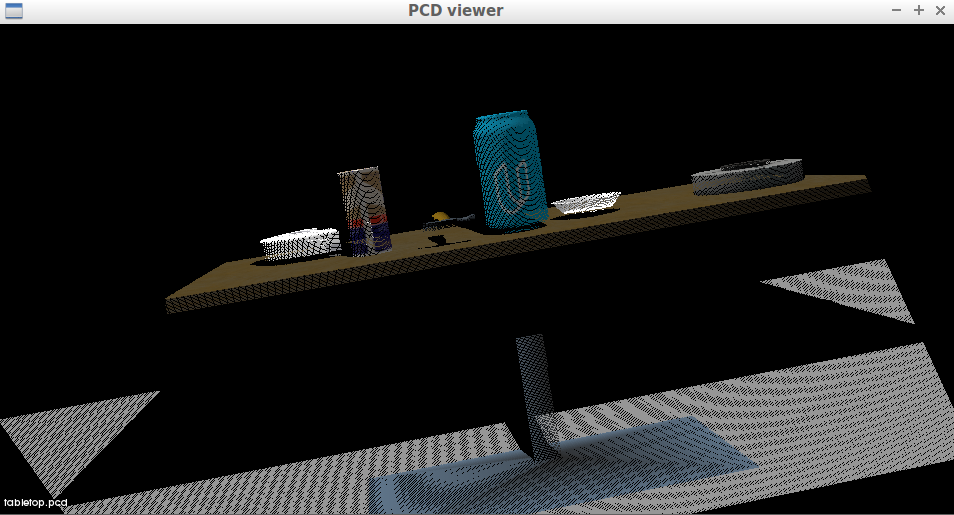
\includegraphics[width=\linewidth]{ex1tabletop.png}
    \caption{Point cloud file from RGB-D camera}
    \label{fig:camera}
\end{figure}

Voxel grid downsampling reduces the density of the point cloud, allowing for faster computations without any loss in the ability for the point cloud data to be used for object recognition later in the perception pipeline. A voxel can be thought of as a three dimensional analog to a pixel. The input point cloud can be divided into a voxel grid by dividing it into cubic regions. To perform the voxel grid downsampling, the points within each cubic region (voxel) are replaced with a single point that represents the average of the points contained within the voxel. By choosing the size of the voxel appropriately, the downsampled point cloud will provide a good approximation of the original point cloud while allowing faster computation in later steps.
For this project, voxel grid downsampling is accomplished using the python PCL library. A VoxelGrid filter object is created from the input point cloud and a filter() function can be run on this object after the size of the voxel is set.

\begin{figure}[H]
    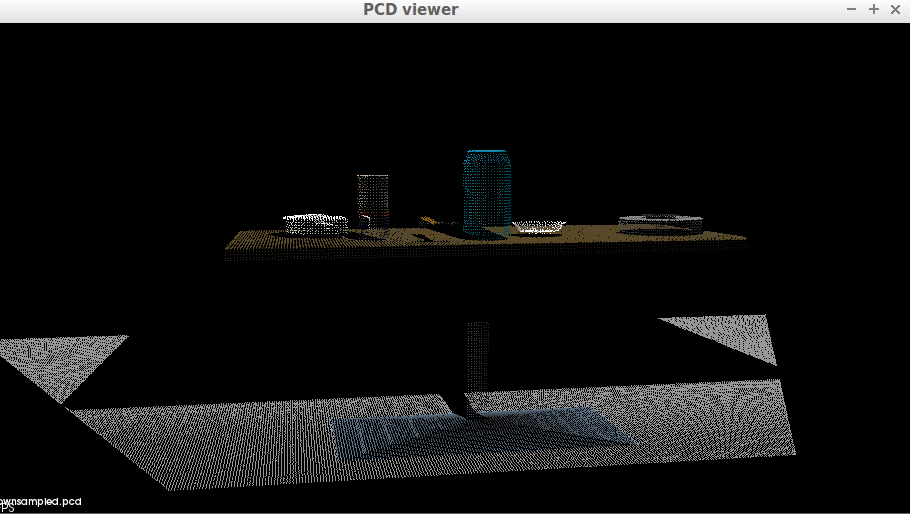
\includegraphics[width=\linewidth]{ex1downsampled.png}
    \caption{Point cloud file after voxel grid downsampling}
    \label{fig:downsampled}
\end{figure}

\subsubsection{Pass Through Filtering}
Because the robot and the table are both stationary for this project, 

\begin{figure}[H]
    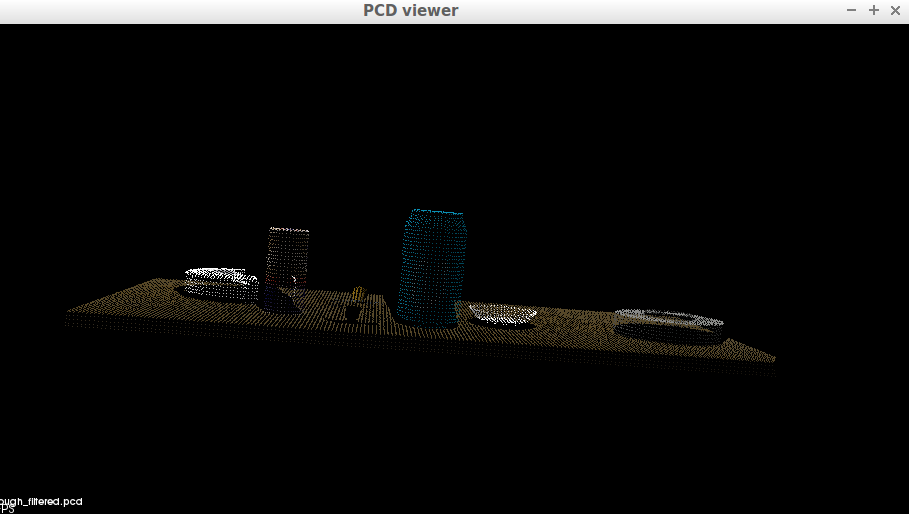
\includegraphics[width=\linewidth]{ex1passthrough.png}
    \caption{Point cloud file after passthrough filtering}
    \label{fig:passthrough}
\end{figure}

\subsubsection{RANSAC}

\begin{figure}[H]
    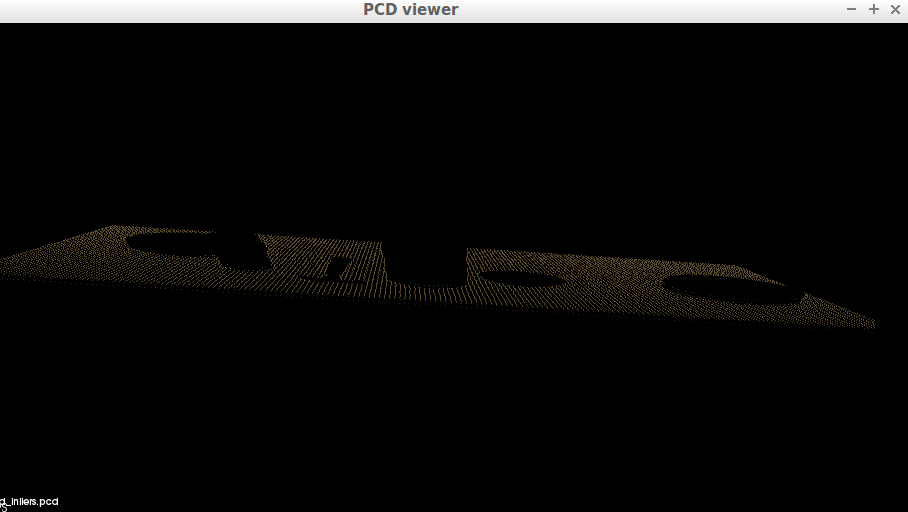
\includegraphics[width=\linewidth]{ex1extractedinliers.png}
    \caption{RANSAC inliers}
    \label{fig:inliers}
\end{figure}

\begin{figure}[H]
    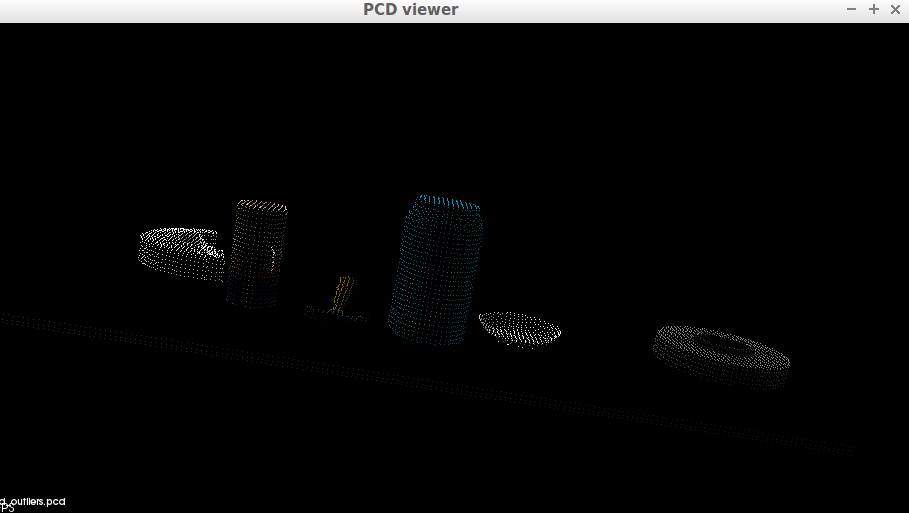
\includegraphics[width=\linewidth]{ex1extractedoutliers.png}
    \caption{RANSAC outliers}
    \label{fig:outliers}
\end{figure}

\subsection{2. Complete Exercise 2 steps: Pipeline including clustering for segmentation implemented.}

\subsection{3. Complete Exercise 3 Steps.  Features extracted and SVM trained.  Object recognition implemented.}


\section{Pick and Place Setup}

\subsection{1. For all three tabletop setups (`test*.world`), perform object recognition, then read in respective pick list (`pick\_list\_*.yaml`). Next construct the messages that would comprise a valid `PickPlace` request output them to `.yaml` format.}


% Spend some time at the end to discuss your code, what techniques you used, what worked and why, where the implementation might fail and how you might improve it if you were going to pursue this project further.  


\end{document}
